\clearpage
\thispagestyle{empty}
\movetooddpage
\addcontentsline{toc}{part}{Fragmentos de um diário\vspace*{-5pt} encontrado}
\part*{Fragmentos de um\\ diário encontrado}

\vspace*{1.5cm}

\emph{Numa noite de novembro (em circunstâncias que não cabe aqui
revelar) achei, na ponte Mirabeau, em Paris, um caderno de capa preta,
lustrosa, de lona, igual àqueles que costumam ser usados nas
mercearias como livro"-caixa. Continha exatamente 126 páginas de papel
ofício recheadas por uma letra miúda, regular, sem rasuras. Leitura
curiosa, por vezes cansativa, passagens obscuras, anotações que me
pareceram estranhas ou mesmo absolutamente impróprias.}

\emph{Fui atrás do proprietário daquele caderno. Fui atrás dele com
perseverança bastante para que minha consciência permanecesse tranquila,
mas por meios suficientemente vagos para que o caderno pudesse ficar comigo.}

\emph{Publico aqui uma seleção de fragmentos dele. Caso algumas
expressões soem desajeitadas, isso se deve inteiramente à minha
tradução. O manuscrito é em francês.}

\emph{Em alguns trechos nos quais a tradução me pareceu perfeitamente
desastrada, adicionei entre parêntesis a expressão exata do texto. De
qualquer modo mantenho à disposição dos interessados o original.}

\movetooddpage

\section{i}

Enquanto narrava o acontecido a M.~D., ele lançou a seguinte
observação, a propósito:

--- Bela experiência!

Só isso fora capaz de entender de tudo o que eu havia dito. Uma
experiência. Tenho horror a esse termo. Serve bem para seus
exercícios de psicologia aplicada. Não tenho como viver com uma folha de
observação na mão. Contornar a vida como um espectador, ajustá"-la ali,
escorá"-la aqui, ajeitá"-la. Entre um arbusto que cresce selvagem e um
jardineiro com tesouras e ideias, minha simpatia de animal vai para o
arbusto, por inteiro.

Contra esses arroubos de psicólogo só tenho a faculdade de esquecer. Mas
a tenho por inteiro. Jamais me obcecou a lembrança de uma mulher
possuída (aliás, minha vida decorre fora do cercado do amor).
Jamais fui perseguido por uma palavra proferida, um sorriso ou
um espasmo.

O que devo fazer com todas essas folhas mortas, que M.~D. chama de
experiências? Se, raras vezes, contrariando minha natureza
introvertida, pude experimentar momentos de felicidade profunda, foi
justamente por ter sabido vivê"-los do jeito que vinham, sem procurar
nada para além ou aquém deles.

M.~D., que é médico, sofre de uma deformação profissional. Toma medidas
preventivas contra a vida da mesma maneira como tomaria contra a febre
tifóide. Reúne experiências na rua da mesma maneira como outrora reunia
observações na clínica, enquanto escrevia para a tese de doutorado. Não.
Essa brincadeira me tira do sério. Não quero prevenir coisa nenhuma e
nem corrigir nada. Ao vento que sopra, ofereço-lhe meu rosto.
Que me penetre como se eu fosse uma árvore na estepe, que me açoite à
vontade e cesse quando bem entender! Melhor ainda se no final das
contas eu ainda estiver de pé! Senão\ldots{}

Ah! Experiências divertidas que penteamos, lustramos, simplificamos e
finalmente colocamos na memória como numa vitrine! Quem sabe? Talvez
ainda sejam úteis! Mas é claro que não! Dentre
todas as avarezas essa é a que eu mais detesto: poupar migalhas de vida
para mais tarde, para a velhice, para os momentos de tédio eventual. Não
consigo fazer esse tipo de economia. Mordo uma maçã na medida da minha
fome: uma vez saciado, jogo"-a fora.

\pagebreak
\thispagestyle{empty}
\movetooddpage

\section{ii}

Acho que suportei com bastante estoicismo toda sorte de humilhações, de
uma só porém fui poupado. A humilhação do fracasso. Fracassamos ao
desviarmos do caminho que queremos seguir ou quando chegamos ao lugar
onde parecia que tínhamos de chegar. Jamais me considerei
fadado a qualquer tipo de caminho. Andei por onde o acaso me levou,
cheguei onde calhou chegar.

Não era em meus gestos visíveis que o essencial se produzia. Os outros ---
amigos, mulheres e adversários --- acompanhavam minha vida baseando"-se
naquela moldura exterior, contentes por poderem ler nas cifras algo
legível talvez só nos grãos.\footnote{No meio
rural romeno, é comum a arte divinatória baseada na leitura de grãos, em
geral de milho, arremessados à terra.} E eu dava risada, sabendo da distância
que havia entre mim e seus cálculos.

Com frequência pensei no destino de um cavalo puro"-sangue que,
levado pelos acasos da vida, viu"-se obrigado a puxar as carroças da
prefeitura, arreado lado a lado com os rocinantes miseráveis do
estábulo. É uma imagem que não me entristece.



\movetooddpage
\section{iii}


%\emph{(poor old self.)}

Quando ela viu que eu não respondia e que sua partida me era
indiferente, E. voltou da soleira da porta. Estava surpresa. Talvez
também estivesse em jogo sua vaidade feminina. Mas
estava sobretudo supresa.

Como assim? Ela me abandona, diz claramente que não me ama, que jamais
voltará a me ver, dando mesmo a entender que outra pessoa, outra pessoa
``muito melhor'' do que eu haveria de ocupar o meu lugar, --- e eu não
respondo, não protesto, não me ergo!

Pobre moça! Com toda a sabedoria que Deus lhe deu, tem a
ingenuidade de achar que todas as coisas devem ter um sentido
neste mundo! Pensava que eu ficaria destruído, porém me vê calmo à sua
frente.

Se ela entendesse que todas essas histórias de amor só têm para mim a
importância de um detalhe! Se soubesse que em nosso romance
encerrado eu fora o tempo todo ausente, sozinho, alheio! Na minha vida
o amor é uma ocupação secundária e por isso minhas derrotas nesse
campo não têm qualquer consequência. Pouco importa a um maratonista
campeão ser derrotado numa luta de boxe. Mas como poderia E. chegar a
tal distinção (mesmo que eu explicasse nesses termos esportivos), ela
que na roleta aposta no amor, e quando perde, perde tudo?

\movetooddpage

\section{iv}

Também passei por crises amorosas, mas embora já sejam velhas e minha
memória possa me trair, acho que no fundo foi sempre outra coisa. Um
certo desgosto por uma vida que pressentia tornar"-se demasiado segura
de si, inerte. Uma certa saudade de romper com toda uma
situação que não era propriamente uma situação, mas apenas um acúmulo
de acontecimentos miúdos que me imobilizavam por sua quantidade e
mediocridade.

Então buscava o amor como quem busca uma janela. E me enganava
redondamente. Até mesmo em 1922, em Lyon. Sim, até mesmo naquela
ocasião.

Pois, na verdade --- e confesso sem tristeza, mas também sem orgulho ---,
nenhuma dessas tais de crises amorosas era suficientemente forte
para que não as pudesse liquidar nos bordéis da Monsieur"-le"-Prince.
Depois, só ficava o resto.

\pagebreak
\thispagestyle{empty}
\movetooddpage
\thispagestyle{empty}

%\begin{vplace}[30]
\begin{center}
\vspace*{-1.9cm}
\hspace*{-1.45cm}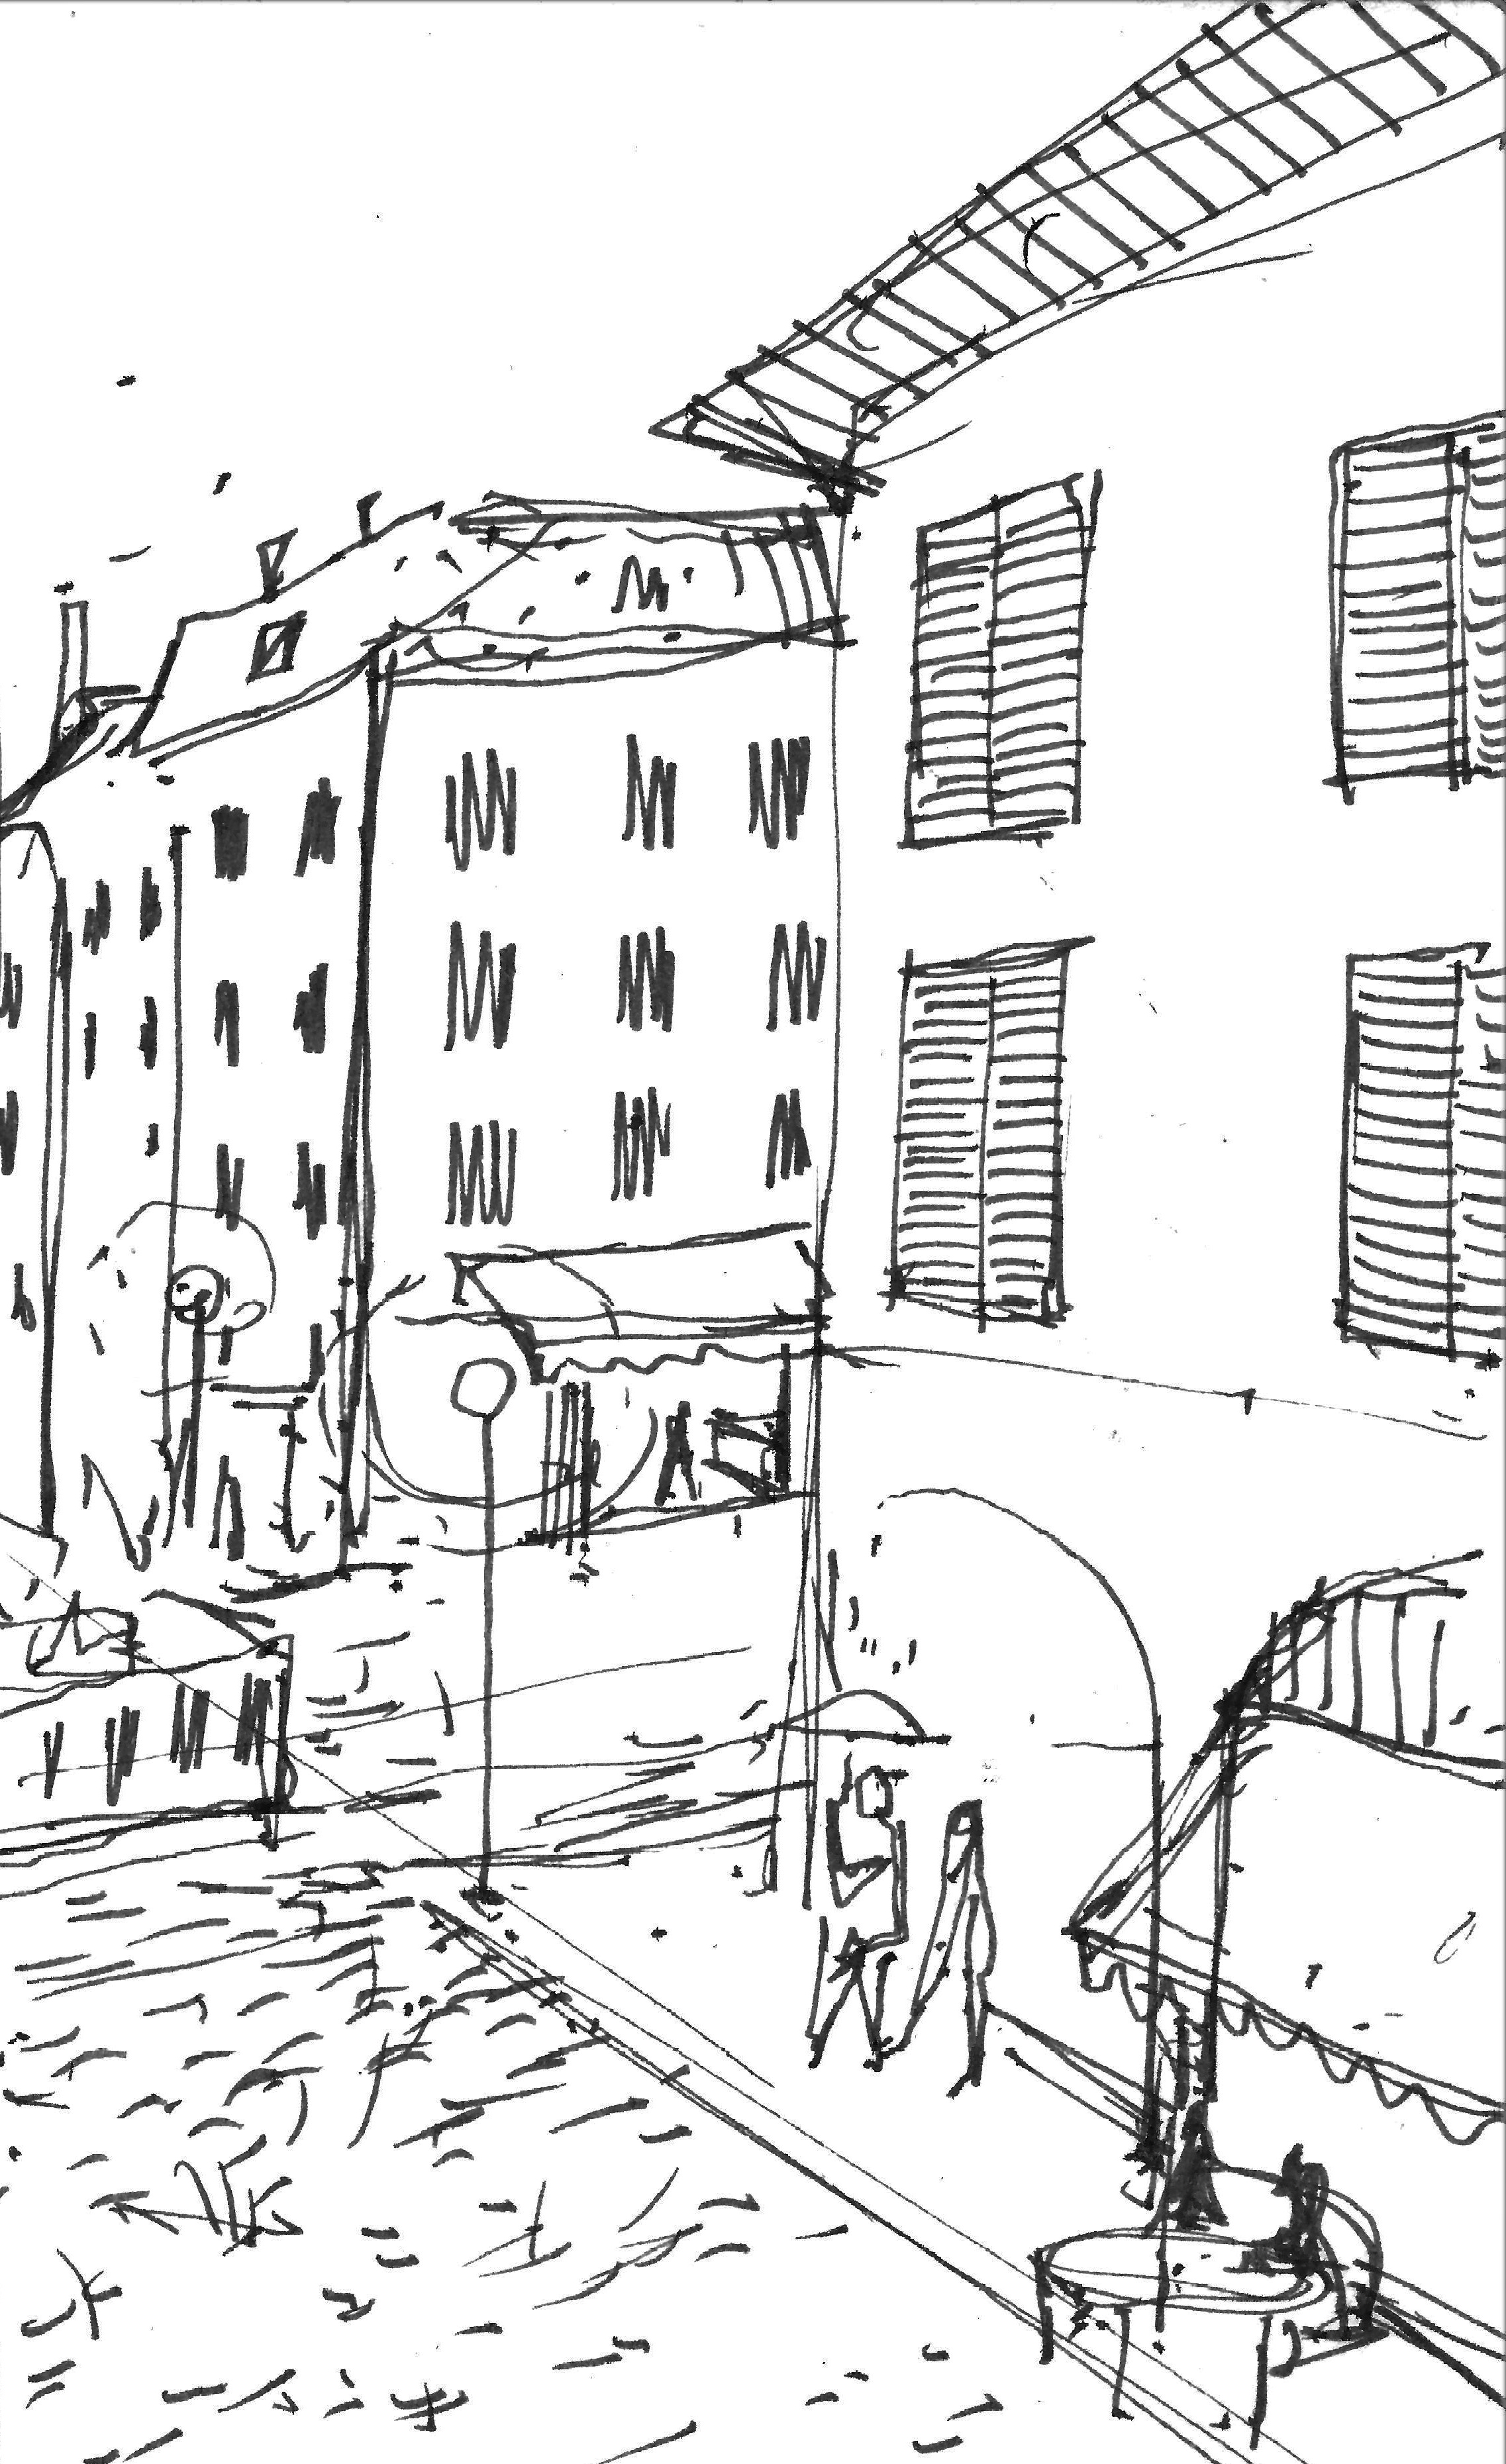
\includegraphics[width=111mm]{./imgs/rua.jpg}
\end{center}
%\end{vplace}



\pagebreak
\thispagestyle{empty}
\movetooddpage
\section{v}

Não acho que tenha alguma vocação especial para a miséria. Observo
apenas que não me incomoda.

Longas noites de novembro, trajetos intermináveis debaixo de
chuva por ruelas desgraçadas do outro lado de Austerlitz, na Bastilha,
na Place du Tertre, para retornar tarde da noite às margens do Sena! A
chuva me penetra como se eu fosse uma viga apodrecida, as luzes das
vitrines parecem irreais, a campainha dos bondes surge ensurdecedora
do alto da rua, detenho"-me como um idiota diante das prateleiras das
padarias, leio os saldos dos açougues, uma bisteca 2,50, um escalope
3,75, continuo andando por inércia, da mesma maneira como me detive, não
desvio das poças, não peço perdão ao atingir um transeunte com o
cotovelo, não evito os automóveis, não penso em nada. E a carícia
recatada (no texto: \emph{paisible}, \textsc{n.~t.}) da chuva que escorre sobre as
faces!

Como poderia explicar, se alguém me perguntasse e se eu tivesse
vontade de responder, como diabos é que poderia explicar minha
profunda tranquilidade nesses momentos? Pois estou longe de ser um
vagabundo ou um resignado!

E nem mesmo acredito na pobreza como um estado de espírito (no texto:
\emph{état de grâce}, \textsc{n.~t.}). O que aconteceu nas primeiras horas do dia
primeiro de janeiro, lá em cima na Sacré"-C\oe ur, foi o que me
comprovou\ldots{}


\movetooddpage
\section{vi}

Mais uma palavra que preciso suprimir do meu vocabulário:
\emph{explicação}. Esse vocábulo não tem nenhum sentido para mim.

Nunca tive crises da alma. Só tive temporadas. E se há explicações para
as crises, para as temporadas não há.

Eu entrava na condição trágica assim como uma planta que deve hibernar.
Tive meus invernos da alma e pronto! Não por isso berrei de
desespero, nem mesmo esperei. O que poderia esperar? O que é que uma
árvore espera em pleno mês de janeiro, toda desfolhada, com o tronco
fendido e os galhos enegrecidos?

Minha única façanha nesta longa existência, única mesmo, foi
compreender a tempo --- embora minha vida seja um fato singular no
desenrolar do mundo, um fato desprovido de algo que o preceda ou que o
suceda --- que meu ser faz parte dos grandes quadros da zoologia.

Crises e explicações se transformam em meras brincadeiras diante dessa
verdade.

\movetooddpage
\section{vii}

%\emph{(now, like so.)}

M.~D., médico e psicólogo, afirma que desprezo minha própria
inteligência.

Não, não é verdade. Coloco"-a no seu devido lugar: isso, sim. Sei que é
hábil e afiada. Mas sei também que a vida (esta vida levada pelo vento,
assediada, desassossegada, que detesto e que amo ao mesmo
tempo) não necessariamente precisa dela.

Logrei realizar a façanha --- e me admiro com o fato de que M.~D., amante
das experiências, não a tenha observado e elogiado --- de não permitir que
minha inteligência funcione em prol de si mesma. Utilizo"-a apenas para
minhas relações com o mundo exterior. É um gesto de boa educação. Mas
ela, para mim, pessoalmente, pouco importa. O tamanho (no texto: \emph{la
grandeur}, \textsc{n.~t.}) jamais foi realizado pela inteligência.

Guardo, para meu próprio divertimento, todas as noções que tornam a vida
possível e conveniente. Justo ou injusto, bom ou mau, bonito ou feio,
moral ou imoral, tudo isso é desprovido de sentido, de verdade, de
profundidade. Não acredito em nenhuma dessas porcarias. Não
conheço nenhum santo moral!

Moralidade e santidade se excluem. Se fosse minha profissão,
iria procurar santos nas minas de trabalho
forçado.\footnote{Na Romênia do entreguerras, era comum que o trabalho executado nas minas de sal fosse realizado por detentos.} Ainda
assim não conseguiria encontrar santos cujos suplícios o código
penal não prevê.

De qualquer modo, sabendo o que eu sei, brinco neste mundo com a escala
de valores que todos acessam. Digo que isso é ruim e aquilo é bom. Que
isso é bonito e aquilo é feio. Admito e reprovo, comparo e chego a
conclusões. E nem mesmo consigo morrer de rir.

Que volúpia seleta! Oh, esse M.~D. que defende os direitos da
inteligência contra mim! Quando terá tido ele semelhante alegria?

\pagebreak
\thispagestyle{empty}
\movetooddpage
\section{viii}

De uma carta enviada por E. (que está em Bordeaux já faz duas semanas):

``Não, você jamais saberá quanto eu te amei, pois vocês, homens, nunca
sabem nada do que está acontecendo. Ninguém sabe nada do que está
acontecendo.''

De maneira que ela também, a doce, suave e loira E., também acabou
descobrindo a verdade. Verdade que consegue exprimir com uma
melancolia que não vale um vintém, mas consegue.

``Ninguém sabe nada do que está acontecendo''? Graças a Deus! Senão
seria pavoroso.

Se vivi minha vida do jeito que ela foi, boa, ruim, me
afoguei em todas as suas humilhações, me submeti a todas as
misérias que conheço e que não conheço, concordei em carregar os
farrapos desta triste existência, foi porque tinha certeza de que
ninguém teria como saber e, mesmo que soubesse, ninguém
compreenderia que no final das contas vou ficar sozinho, mais sozinho
do que uma estrela no céu, mais sozinho do que um boi na cocheira.

A tragédia de ser incompreendido? Não a conheço. Querem dizer o prazer,
a paixão, o êxtase de ser incompreendido. Sentir"-me único,
entrincheirado dentro de mim, impenetrável, sozinho com as próprias
superstições, os próprios símbolos, sinais, ídolos, saber que a vida
que vivo não é vivida por mais ninguém neste mundo, que mais ninguém
pode nem mesmo imaginá"-la, levar comigo esse mistério do qual não podem
me separar, nem que o revele aos berros em praça pública, nem que
o grite no palco de um teatro, nem que o distribua impresso em
cartazes\ldots{} Meu Deus! Pergunto"-me como posso ter merecido tanta
felicidade!

Eu talvez também tenha tido momentos de efusão quando me sentia
oprimido pela solidão, quando quis dizer a alguém simples palavra
que pudesse ser compreendida, busquei por vezes sinais de
comunhão nos olhos do outro, nas suas palavras e nos seus silêncios. Mas
não passaram de breves momentos de ingenuidade de que aliás não me
arrependo, pois não me arrependo de nada, mas que não me levaram a lugar
nenhum. Amigos e amantes permaneceram em algum lugar ao meu lado, presos
a palavras que não disse, enganados por uma sombra que eu não era. No
final fiz de tudo para evitar equívocos. Falei com sinceridade. Não
escondi. Não trapaceei.

Não, não. Há dimensões (no texto: \emph{grandeurs}, \textsc{n.~t.}) que não se
pode recusar nem abdicando. A minha solidão é uma delas.

\pagebreak
\thispagestyle{empty}
\movetooddpage
\section{ix}

Troquei de pessoas como quem troca de chapéu, procurei sua amizade,
conversei com elas, fiz com que falassem comigo e no fim abandonei"-as
no meio do caminho, pois não me interessavam mais, nada nelas
correspondia à minha busca, eram todas iguais às anteriores e
iguais às que vieram depois delas, puídas, previsíveis, monótonas.

Algumas eram inteligentes. Jovens, com detalhes pessoais curiosos,
as mais diversas histórias. Depois de um tempo de duração variável,
mas jamais demasiada, percebia como todos aqueles brilhos
empalideciam. Eram qualidades mais ou menos grandiosas. Mas eu, que não
sou psicólogo, não posso empregar ``mais ou menos''. Escapam"-me os
termos justos de comparação. O que é preciso, ou melhor,
absolutamente necessário à expectativa que tenho de cada instante é a
feição única de um fato, de uma pessoa, de uma palavra. Não peço a
ninguém que seja bom ou mau, bonito ou feio, canalha ou anjo. Peço"-lhe
apenas que seja algo que exista uma única vez.

Raramente tive a alegria de tais encontros, mas tive. (O escocês de
Poulmanach\ldots{}) Todos os outros não passaram de acréscimos ou
subtrações de uma alma padrão. X é mais inteligente que Y, mas Y é mais
sutil que Z, que, por sua vez, é mais espiritual que X.

Não, não e não. Tais variações me matam de tédio. De que adiantam
nuances e definições e pontos de vista? Junte"-se a mim deste lado, meu
senhor, caso o senhor se componha de um material inédito surgido com o
seu nascimento! Se não, dê o fora!

Busco nas coisas e nas pessoas seu som próprio. Só me interessa aquilo
que tenham de irredutível. Irredutível! É a minha única maneira de
sentir a eternidade.

\pagebreak
\thispagestyle{empty}
%\movetooddpage
%\thispagestyle{empty}
%
%%\begin{vplace}[30]
%\begin{center}
%\vspace*{-1.9cm}
%\hspace*{-1.45cm}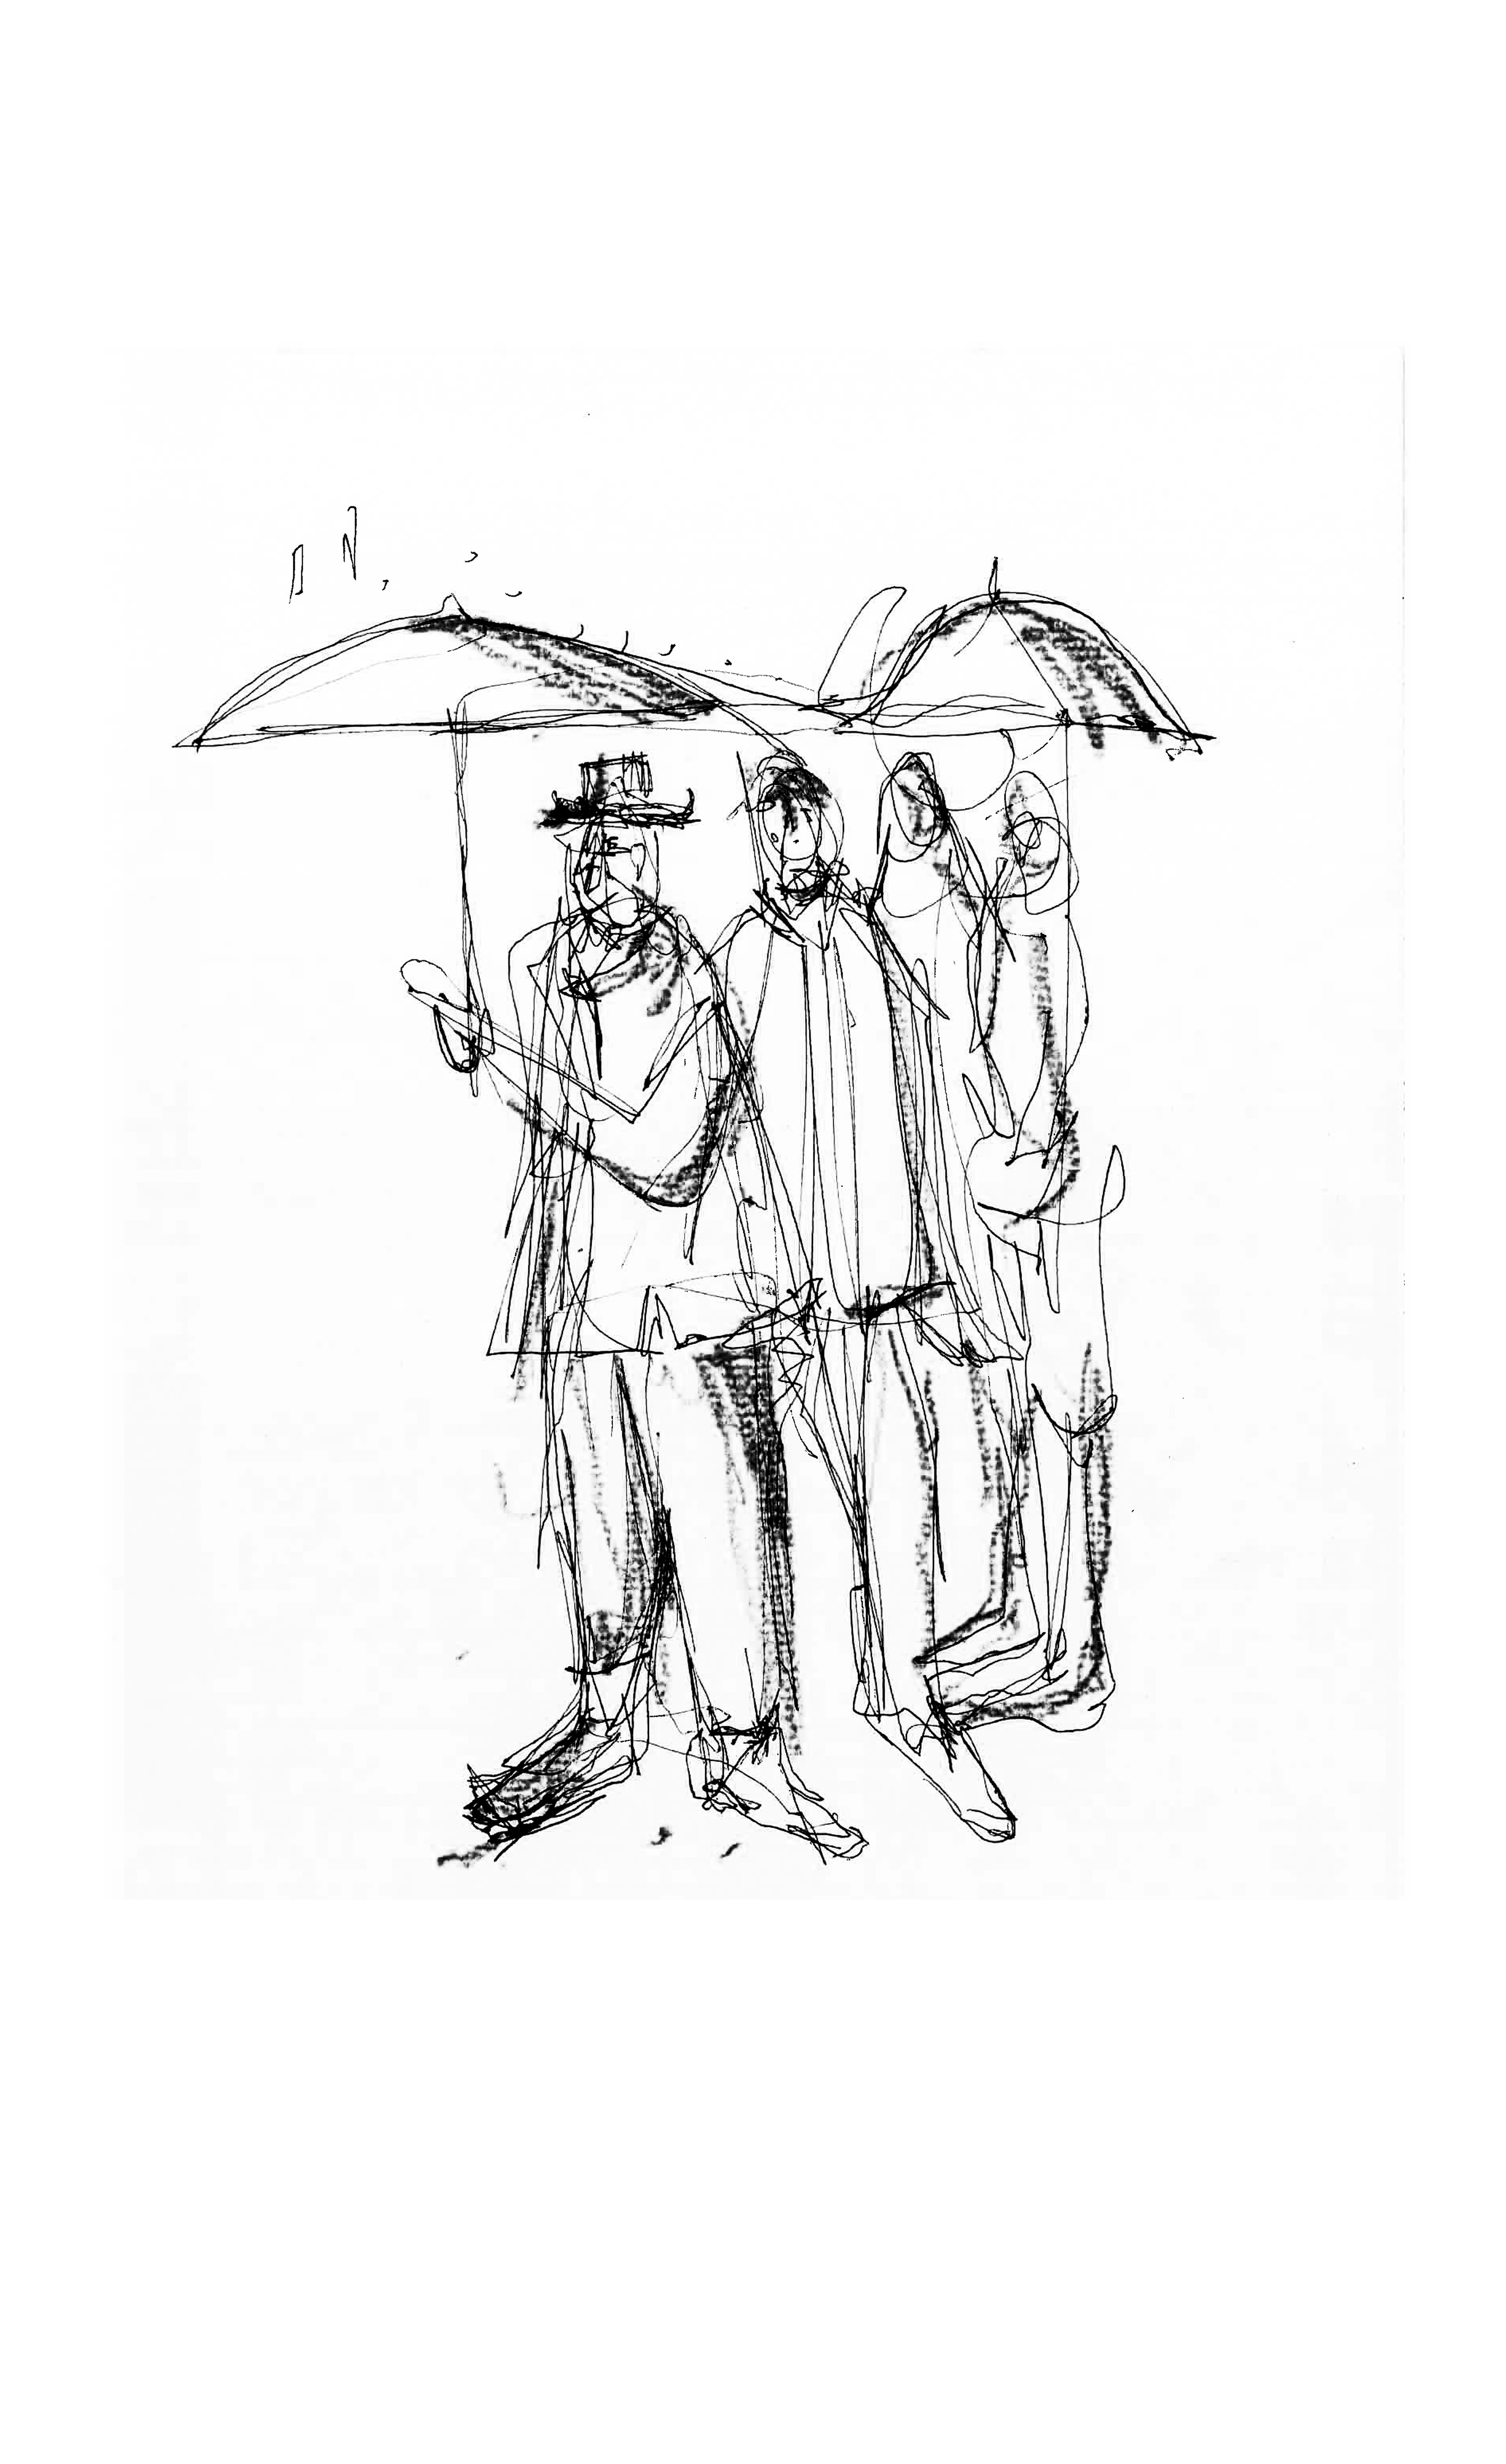
\includegraphics[width=111mm]{./imgs/chuva.jpg}
%\end{center}
%%\end{vplace}

\movetooddpage
\section{x}

Não foram numerosos os momentos em que conheci Deus de frente. Não sou
místico, e raramente fui tomado por algum êxtase (no texto: \emph{état
de grâce}, expressão que reaparece várias vezes e em diversos trechos do
caderno, \textsc{n.~t.}).

Ademais, além de um agudo senso de pecado, pergunto"-me o que é
transcendental no meu sentir. Minha ideia de Deus é angulosa, fria por
vezes. Mas o que me estremece diante dela é justamente a sensação de
irredutível que procuro em vão em outras partes.

Ser um, único, único no absoluto, para além de qualquer relação, acima
de qualquer relação, essencialmente único, irredutivelmente único.

Sempre que a vida me esmaga socorre"-me essa sensação inabalável de Deus.

\pagebreak
\thispagestyle{empty}
\movetooddpage
\section{xi}

Faz tempo que desisti da biblioteca. Às vezes ainda vou lá por
necessidade, assim como se leva bolo para festa. Estou trabalhando. Não
tenho mais paixões literárias, mas apenas prazeres, ou satisfações, ou
tédios.

Mantenho, porém, dentre minhas antigas paixões, uma grande aversão:
Descartes.

Já disse, acho (pois é uma das minhas mais firmes verdades), que não
sou uma pessoa moral, e caçoo de tais definições. Mas acredito em loucos
e em heróis e em santos. Odeio esse tal de Descartes, pois ele não só
não fazia parte daquela corporação, como também jamais teve, não, jamais
pôde ter o calafrio de pressentir a santidade. Era um jardineiro.

\pagebreak
\thispagestyle{empty}
\movetooddpage
\section{xii}

A moça que me interpelou em frente à praça Vaugirard não sei como era.
Mal a vi quando passei do seu lado, atirando"-lhe na cara a recusa:

--- Não tenho dinheiro, senhorita.

(Engraçado é que ela talvez nem tenha acreditado em mim!) Mas era alta,
e isso, apesar de tudo, fui capaz de perceber. Devia ser morena.
Apertava com força, em torno do seu corpo delgado, uma espécie de trapo
preto, uma vaga espécie de capa, e tremia tanto que tive a impressão de
ouvir seus dentes batendo dentro da boca. Embora sua voz talvez não
fosse muito diferente da dos mendigos em geral, ela me comoveu. Talvez
por causa de sua juventude. Devia ter uns 20 anos. Acho que era bonita.

Sou um tonto, talvez, e ridículo também, pois eis que o ocorrido não sai
da minha cabeça. Algo perturba o meu trabalho esta noite, e os livros à
minha frente parecem uma piada de mau gosto. Decididamente, não sou um
filósofo: essa moça consegue paralisar o mundo inteiro! Repito para mim
mesmo que tudo não passa de um profundíssimo comprometimento, que tudo é
miserável e mesquinho e abjeto uma vez que isso foi capaz de acontecer.
Será que poderia acusar o universo de algo mais humilhante do que os
olhos da moça de há pouco, que me pediu (provavelmente para que a ironia
do acaso fosse ainda mais áspera) que lhe desse dinheiro? Se esta
noite eu me encontrasse no dia do Juízo Final e fosse a minha vez de me
pronunciar, acho que mandaria ao diabo todas as minhas teorias
filosóficas e contaria o que vi 15 minutos atrás. Seria suficiente,
mais do que suficiente para que a terra fosse amaldiçoada.



\movetooddpage
\section{xiii}

Juízo Final? Acredito sinceramente nele, desesperadamente. É a desculpa
de todas as minhas desistências de hoje, é a força da minha paciência de
sempre.

Aceito os acasos do jeito que vêm, acredito nas pessoas da maneira que
se apresentam, cumpro meu trabalho do modo que calha. Cada dia morde um
pedaço do meu ideal de grandeza (no texto: \emph{grandeur}, \textsc{n.~t.}).
Jamais fiz nada sem defeito, sem rasura, sem caráter provisório. Sim,
declaro tudo isso sem vergonha nem humildade, mas com a dor aferente a
tamanha confissão. Hoje desisti de uma ninharia, amanhã terei desistido
de outra ninharia, consciente do pecado da imperfeição, convencido de
que cada uma dessas mutilações, por menores que sejam, desorganizam por
completo a existência. De maneira que me distancio sem parar da estrela
em que acredito.

Deus sabe que não me submeti ao suplício de maneira leviana, que em cada
uma dessas pequenas ``adaptações à vida'' paguei muito caro, que de
cada uma das derrotas me desviei bem, embora na direção delas um
caminho mais fácil me conduzisse. Mas, sempre que capitulei,
impuseram"-me a trégua e minha rendição foi condicionada. Sabia estar
assinando um papel sem valor. Sabia que a batalha seria um dia retomada,
que todos os redutos perdidos numa guerra limitada haveriam de ser um
dia reconquistados, num só assalto, num só instante.

Aguardo esse chamado com a sensação de que todo o resto é diminuto,
secundário. Nada tenho do caráter de um procurador, não sou vingativo,
não acredito na justiça, mas não posso desistir desta vida por um vintém
em troca. Em algum lugar tenho que imprimir o peso da minha passagem
pela terra. Juízo Final, tenho tempo o bastante para aguardá"-lo.

\pagebreak
\thispagestyle{empty}
\movetooddpage
\section{xiv}

%\emph{De uma viagem à Normandia}

Esse sol violento, esse litoral lamacento de Fécamp, praia que se
estende monótona por quilômetros sem fim, ar com cheiro de grama
molhada --- de que espécie de consciência perdida, própria de um animal,
brota o contentamento de reencontrar tudo isso?

Entre Montigny e Vinmes, nosso caminho foi interrompido por cinco
minutos até que um plátano, cortado, caísse. Haviam"-no serrado desde a
raiz e agora esperavam que se rompesse sozinho, sob seu próprio peso,
das últimas fibras que ainda o mantinham ereto. Operários, motoristas e
pedestres se distanciaram respeitosamente, formando um espaço vazio ao
seu redor, num raio de 50 metros.

Caiu bonito, devagar, descrevendo um arco de estrela cadente, até se
chocar maciço contra o chão, fazendo reverberar longe um barulho, de
início surdo e, depois, amplo, vibrando entre os horizontes como se
dentro de uma concha.

Naquela queda havia algo de supremo e glorioso, que invejei, sabendo que
jamais seria capaz de me separar de coisa alguma com a mesma
concórdia do tronco de plátano, estendido de viés em cima da estrada.

Precisava entender que aquilo também é uma espécie de morte, certamente
a mais bela e inacessível a nós, que morremos sem dignidade,
contra a nossa vontade.

\asterisc

Em Dieppe, num bar do porto, com marinheiros e mulheres perdidas, vi
passada meia"-noite uma mesa nos fundos com um casal estranho. Ele
bêbado, sujo, falante, conversando com os vizinhos de mesa; ela morena,
pálida, muito elegante, observava"-o quietinha, sem contradizê"-lo em nada
e esperando não sei o quê. Vez ou outra, o homem a deixava e ia dançar
com as mulheres do boteco. Ao retornar, batia generosamente nos seus
ombros e ela dava um sorriso triste, não resignada, mas feliz, de uma
cálida felicidade interior.

Que mistério escondia o fato de estarem juntos? Que drama ou que
imaginação pulsava entre eles, unindo"-os?

Não sei, e alegro"-me por não saber. Há algo de majestoso no silêncio e
na ausência das pessoas. Por isso prefiro um símbolo a uma explicação.

\asterisc

Passar com a velocidade de um automóvel em frente a uma janela que se
abre, deixar para trás uma mulher que havia parado justamente para nos
observar, percorrer ao anoitecer a rua vazia de uma vila, na qual atrás
de persianas fechadas ardem luzes mortiças, flagrar vozes e levar
conosco um nome gritado na soleira de uma porta\ldots{}

Nada me dá com maior acerto a sensação da minha solidão, da inutilidade
de toda experiência, da minha desimportância pessoal, eu que me vejo
reduzido a conhecer a mim mesmo e mais alguns enquanto a terra é
habitada por um bilhão e meio de pessoas, mais alguns milhares de
bilhões de outros animais e plantas.

Prometo pensar, num dia vindouro de tristeza, na rotação dos astros. De
todo modo, prometo pensar naquele senhor de fraque e cartola que
contava na praça Saint"-Maclou, em Rouen, as barras da grade em frente à
igreja.

\asterisc

Duas horas em Havre, de madrugada no porto, debaixo de uma garoa
rápida, ampla, de cabeça descoberta, de casaco aberto, os olhos fitando
ao largo as ondas que iluminavam bruscas não sei como e se apagavam.

Um dia vou conhecer a insensibilidade das pedras e das correntes do
porto, cujo sossego sinto que tem certo parentesco comigo.

\asterisc

Na catedral de Gisors, onde entramos para contemplar vitrais do
século \versal{XVII} às quatro da tarde, hora desprovida de mistério, sem
significado, encontrei uma jovem senhora ajoelhada debaixo da
cúpula. Estava vestida com roupa de primavera, parecia muito bonita e
não ergueu a cabeça enquanto passei ao seu lado.

No guia, encontrei essas duas linhas:

\emph{Gisors. 2650 habitantes. Localidade rural. Vinhedos e indústria
animal.}

Gosto da indiferença da informação, de seus termos frios, impessoais e
abstratos. Nenhum guia no mundo jamais registrará a existência daquela
mulher dentro da catedral.

\asterisc

Entre Havre e Rouen, D.~L. desceu do automóvel, carregou o revólver e
matou um galo a tiros.

--- Estou com fome, disse"-nos.

Penso com prazer que, em algum lugar, existe um proprietário que foi
lesado e que, em algum outro lugar, um texto de lei que foi violado só
porque D.~L. estava com fome.

Nem tudo está perdido enquanto ainda formos capazes de um gesto natural.

\asterisc

Coelho ou esquilo, não sei que animal cruzou o meu caminho de
madrugada na estrada secundária rumo a Bolbec, junto a uma ponte onde
havíamos parado para trocar uma roda.

Havia chovido e pairava um cheiro de planta esmagada. Vi apenas os seus
olhos, cintilantes, precisos, que nada indagavam. Fitamo"-nos um ao
outro, de animal para animal, e me alegrei por ser naquele momento
igual a ele, na minha consciência e na dele.

\pagebreak
\thispagestyle{empty}
\movetooddpage
\thispagestyle{empty}
%\begin{vplace}[30]
\begin{center}
\vspace*{-2cm}
\hspace*{-1.35cm}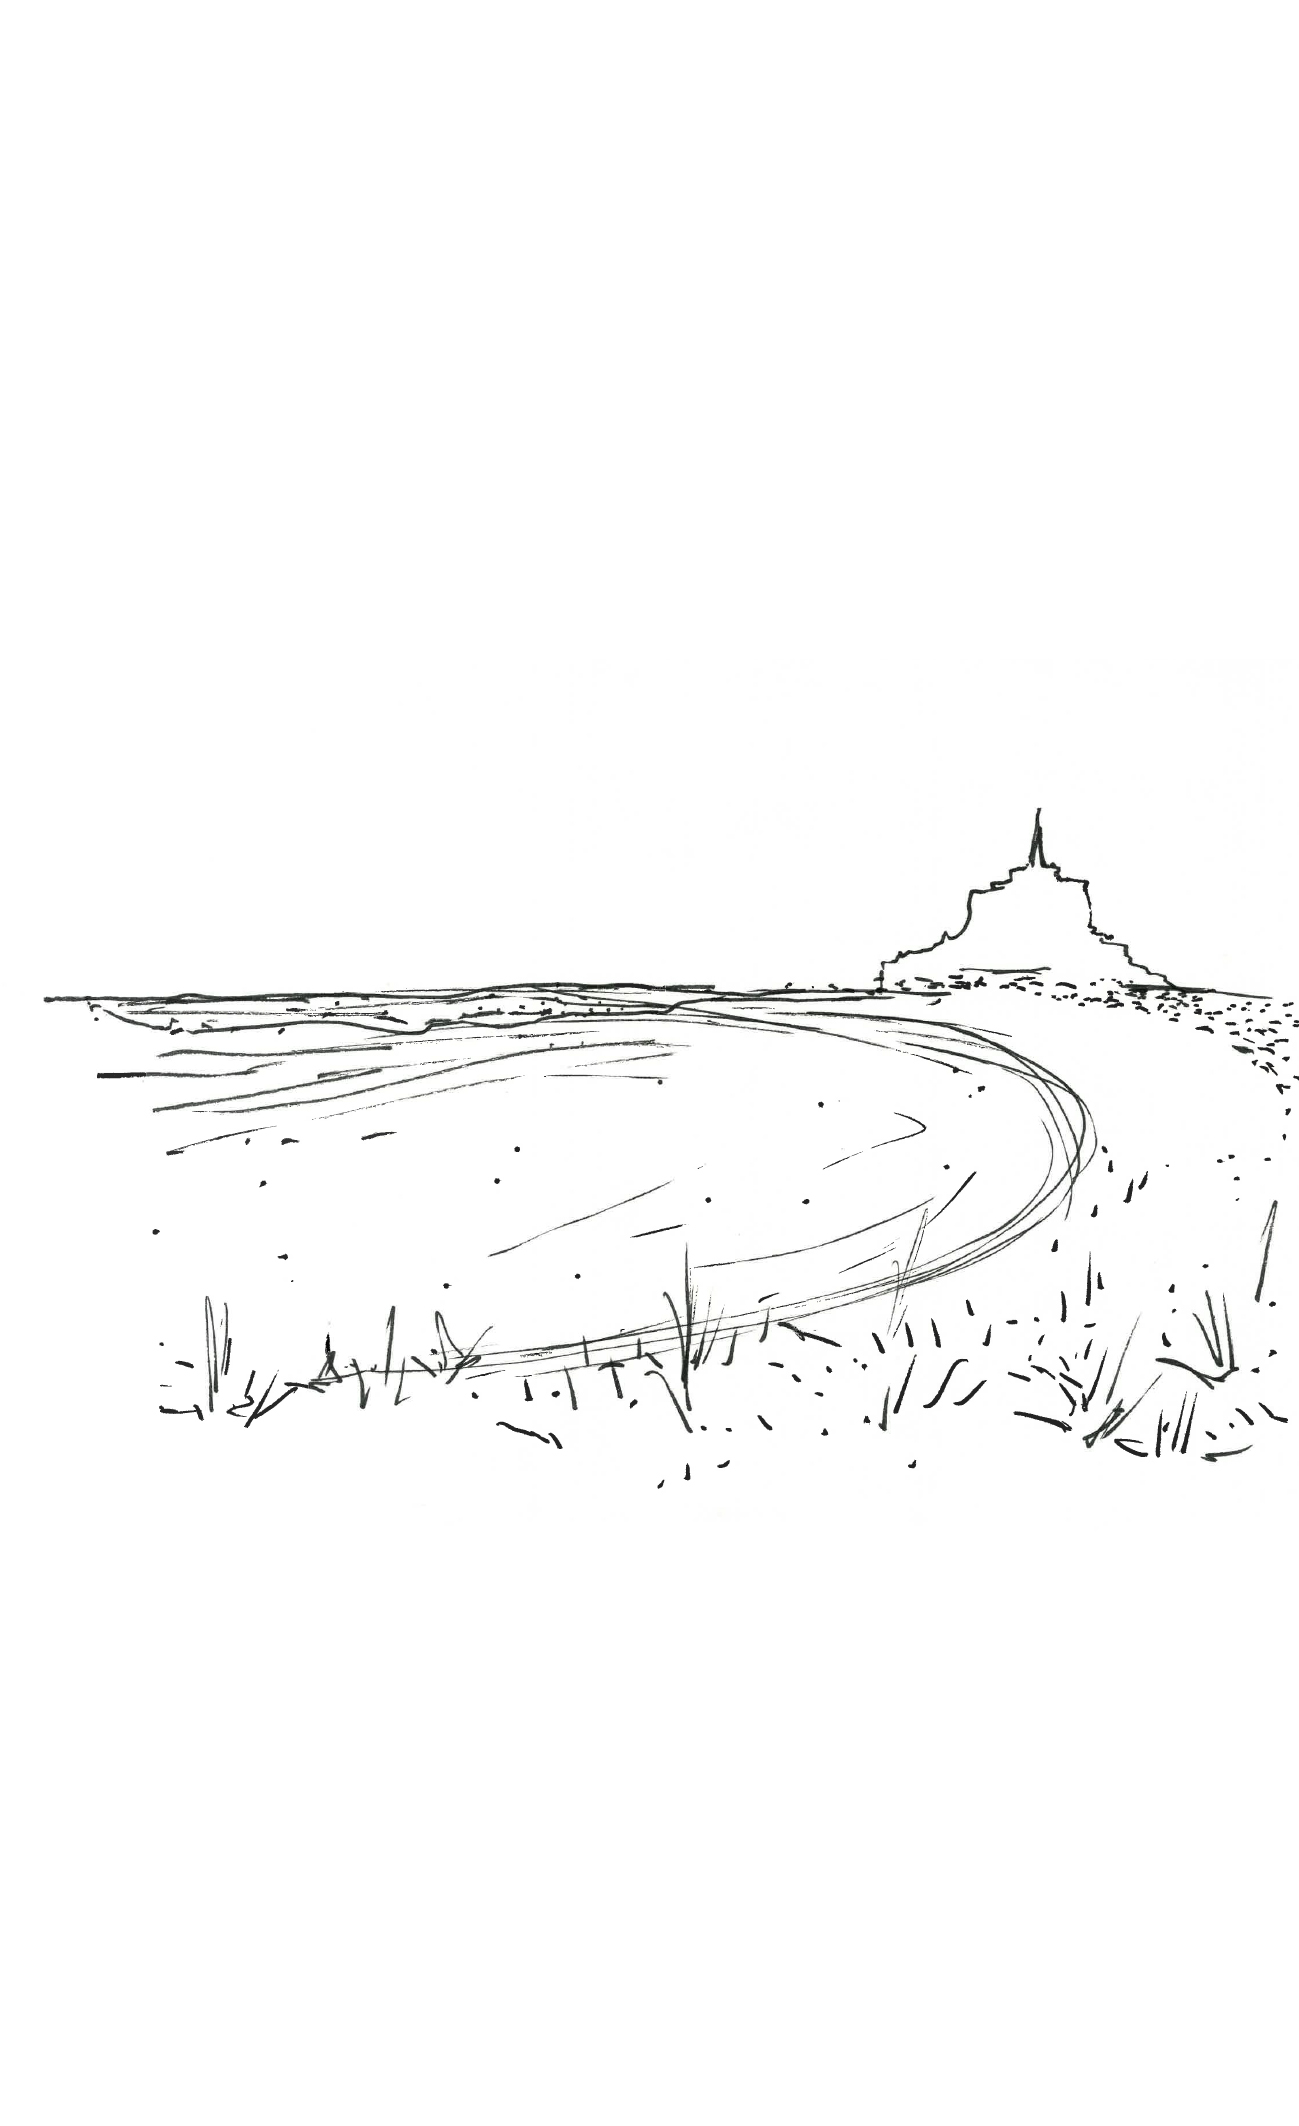
\includegraphics[width=111mm]{./imgs/praia.jpg}
\end{center}
%\end{vplace}

\pagebreak
\thispagestyle{empty}
\movetooddpage
\section{xv}

Despertar no alvorecer do dia, depois de uma assim chamada ``noite de
amor''! Uma mulher ao meu lado --- desconhecida ---, os lençóis
desgrenhados, o braço pendendo na barra da cama, feita de um latão
gelado\ldots{}

Não conheço e jamais conheci a volúpia do cansaço, a pachorra dos
membros à espera do sono, a camaradagem entre dois corpos saciados, mas
apenas um gosto violento por terminar, uma repulsa obstinada pela mulher
ao lado, inútil, trivial, uma necessidade imediata de estar sozinho.

Fico então na espera, com olhar impassível, de capturar a primeira
sombra azul do sol na janela, a primeira luz do dia que venha colocar
ordem nessa perdição.

Um dos sinais indiscutíveis de sua má qualidade anímica é o fato de que
nenhuma das minhas mulheres sentiu, naquele momento, que não existia
mais, aferrando"-se, com alegria inconsciente, ao peito de um homem que
deixava de ser um amante para se tornar um fugitivo.

Pus"-me a refletir de novo sobre a dignidade das árvores, que se amam sem
efusão, num abraço que consome tudo e não deixa rastro.

\movetooddpage
\section{xvi}

Não tenho respeito nenhum por paixões que não incluam um quê de
hostilidade. É o seu princípio viril, lúcido e permanente. É o único
capaz de existir apesar de qualquer visão pessimista, imparcial e nua
sobre a vida e as pessoas.

Talvez devido a um defeito da imaginação, ou talvez a um
sentimento bíblico primário, diante de toda mulher amada me vejo como
se diante de um animal de outra espécie. Jamais fiz com elas, nem mesmo
a título de diversão, tentativas de compreensão mútua.

Apenas O., a morena baixinha e decidida de Talloires, em 1926, encarou a
situação com lealdade e resignação. Não mexia nos meus papéis, não fazia
perguntas, não tentava entender. Durante o dia, ela se transformava em
algo que existia independente de mim: admirava"-a, espichada nua no
terraço, com um sorriso mal desenhado. Ficava lá como um lagarto, com
suas alegrias, suas preocupações, seu horizonte de fenômeno natural e
distinto.

Era à noite que descobríamos um ao outro, com a faísca de fascínio
necessária a toda alegria e uma sensação precisa de que aquilo que
ocorria entre nós dois envolvia no máximo as leis gerais, e de modo
algum a nossa pessoa.

Seria grande desilusão constatar, em algum momento, que minha amiga
O. se tornara uma verdadeira amante. Que decadência!

\movetooddpage
\section{xvii}

Por vezes digo para mim mesmo diante da multiplicação dos
sinais visíveis da minha decadência (botas furadas, aluguel
atrasado\ldots{}) que ainda dá tempo para acordar, retomar as rédeas
dessa existência e pôr finalmente ordem em mim como num armário cheio de
livros. A consciência dos meus ancestrais, camponeses normandos, que
lutaram com a terra e acumularam fortunas sedimentares, pela alegria e
teimosia de acumular, renasce então em mim.

Mas talvez tenha existido entre eles algum marinheiro que viajou anos a
fio por oceanos hostis e amistosos, indiferente à passagem do tempo e
esperando, com um coração apático no peito, grandes tempestades e
grandes calmarias.

Não, não há nada a fazer contra as minhas aptidões de vegetal, e essa é
a única coisa da qual me orgulho, eu, que não me orgulho de nada!

\movetooddpage
\section{xviii}

E se ao menos pudesse me desvencilhar dessa sensação de que
tudo acontece com meu consentimento, com minha participação
inconsciente, essa sensação de uma responsabilidade perpétua.

Não consigo me dessolidarizar de nada, tenho a impressão de que seria
justo ser punido pela chuva que cai lá fora, pela transformação da
noite em dia e do dia em noite, pelo correr do Sena. Acontece de
dizer, à noite, da minha mansarda na Porte de Versailles, quando abro a
janela que dá para esta cidade, de onde vem o ruído surdo do metrô e a
melodia desengonçada de um acordeão, acontece de dizer que, através
da minha mera presença passiva no mundo, colaboro com isso tudo.

\pagebreak
\thispagestyle{empty}

\movetooddpage
\thispagestyle{empty}
%\begin{vplace}[30]
\begin{center}
\vspace*{2.5cm}
\hspace*{-1.2cm}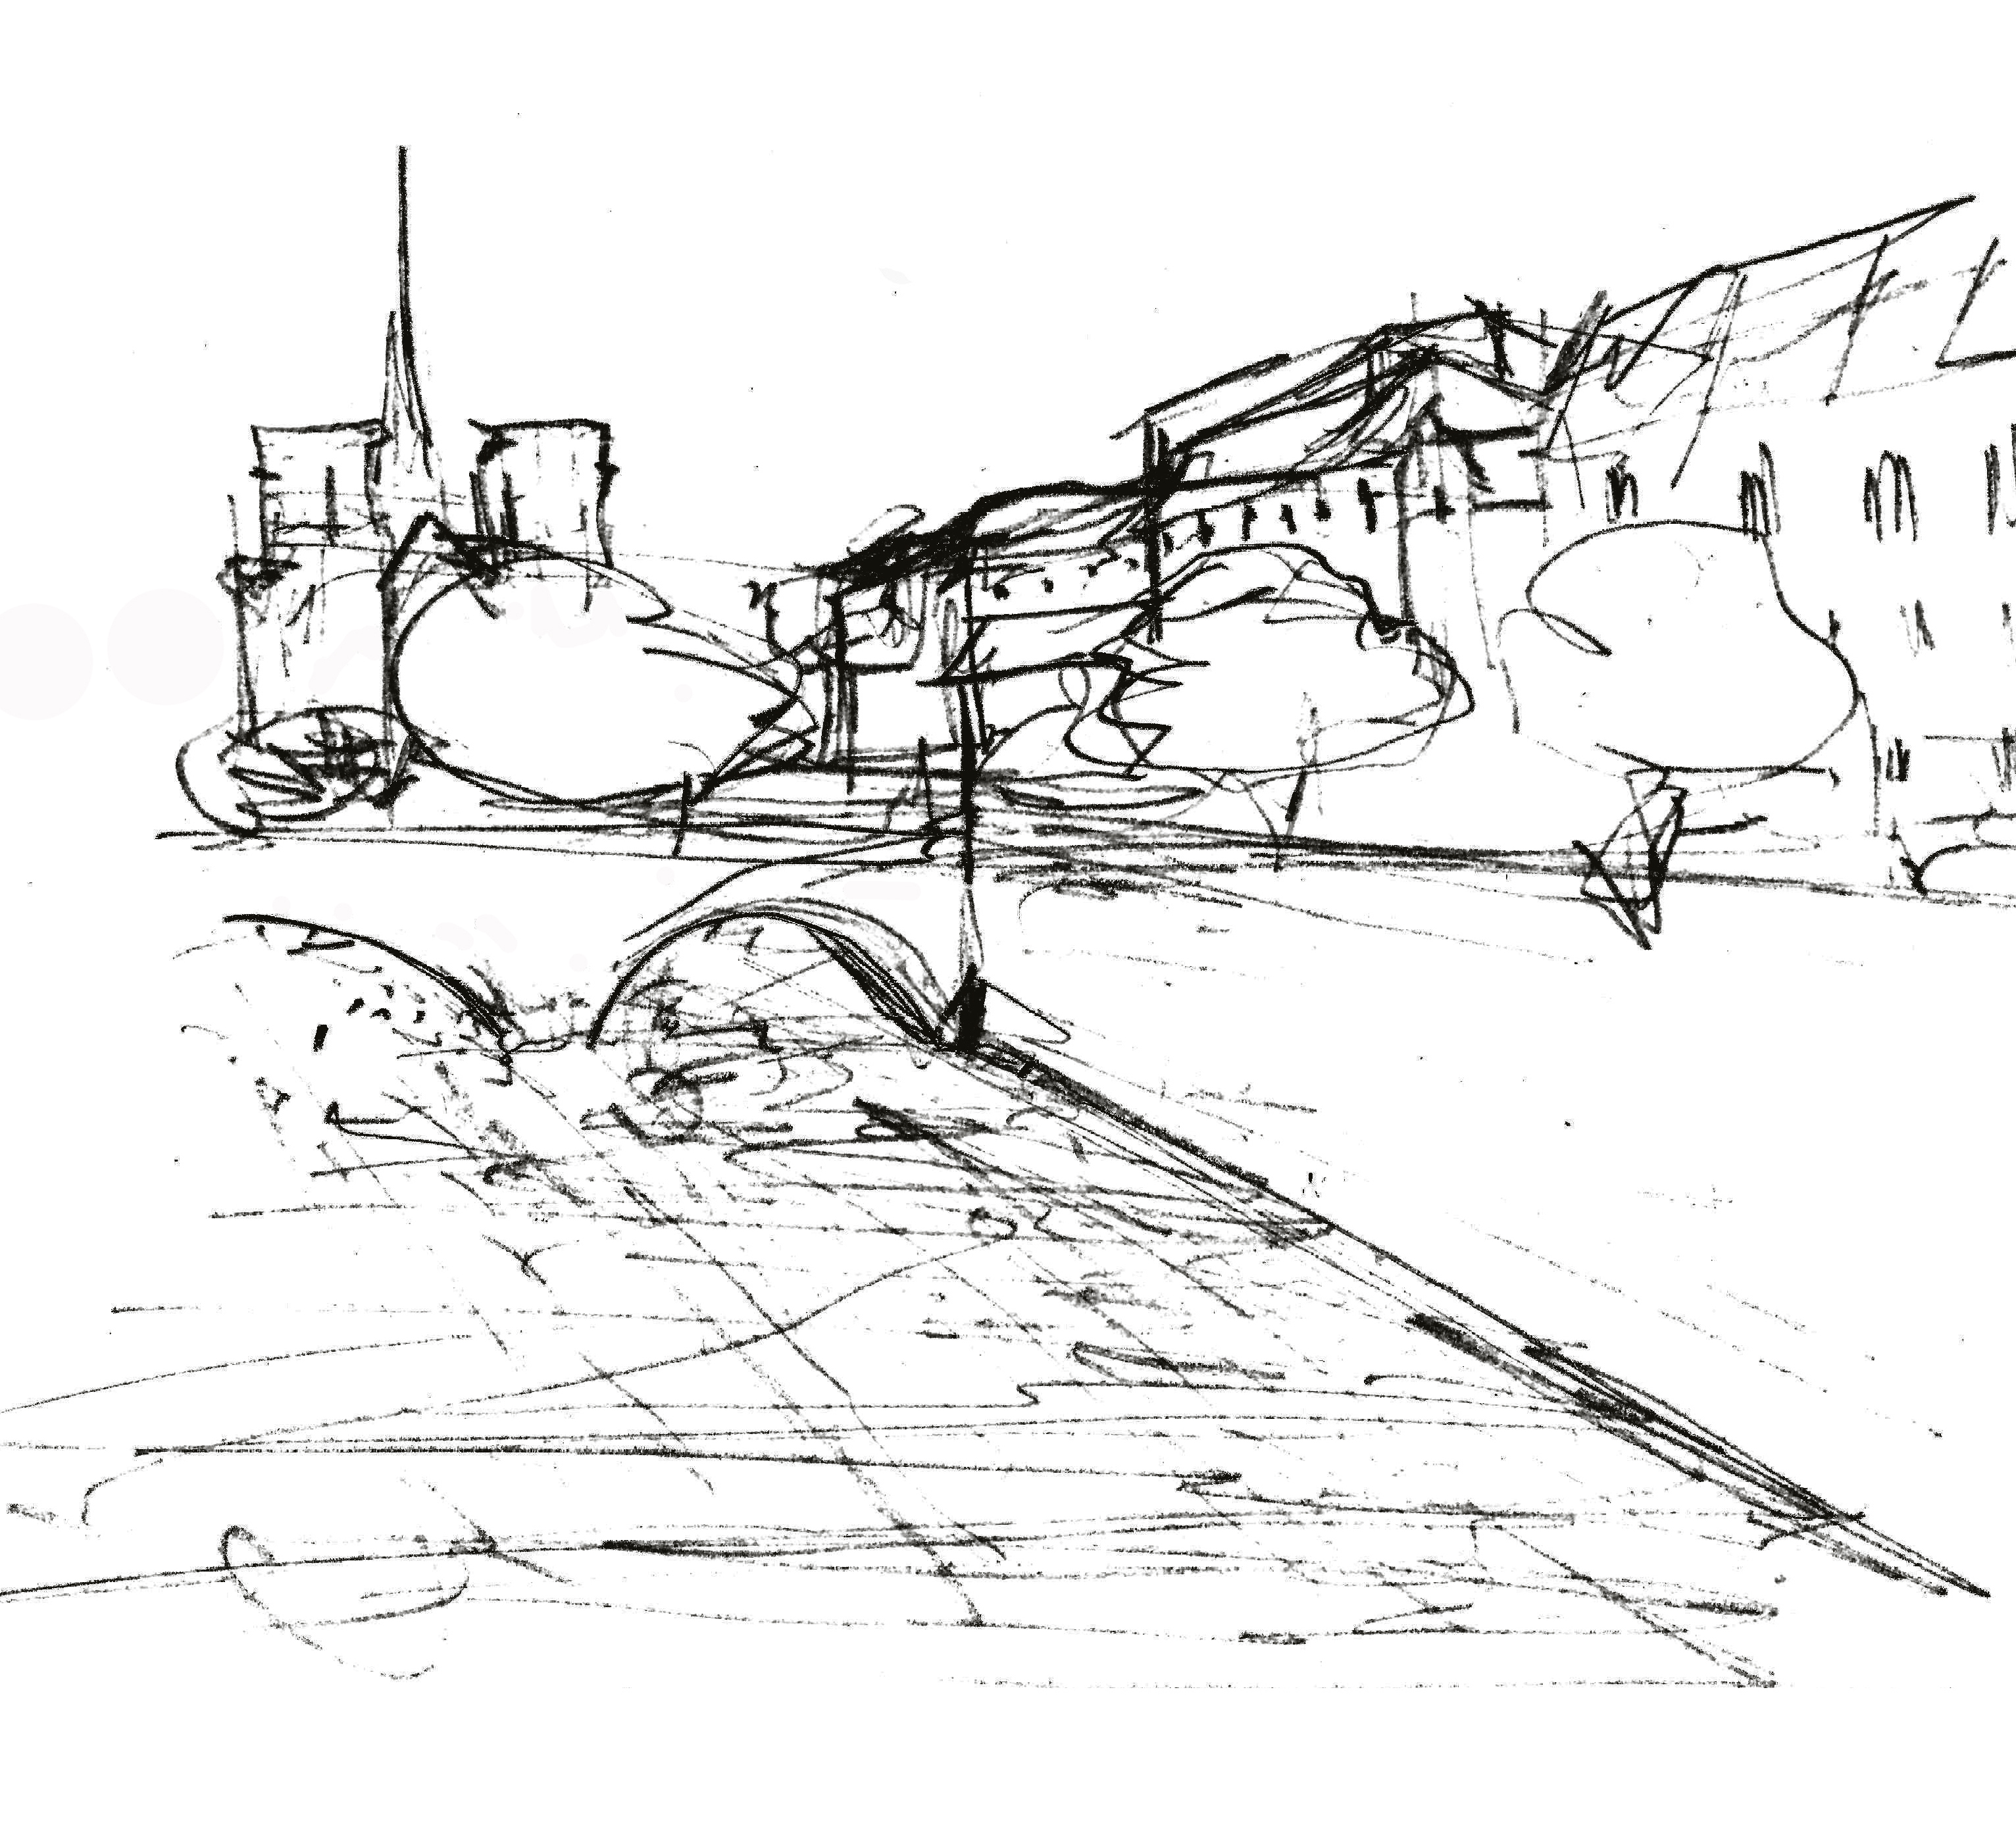
\includegraphics[width=111mm]{./imgs/canal2.jpg}
\end{center}
%\end{vplace}


\pagebreak
\thispagestyle{empty}
\movetooddpage
\section{xix}

Se os caminhos externos não me estivessem todos interditados, será que
encontraria com tanta facilidade os caminhos internos?

Não é acaso que eu seja daqueles que ficam na fila do guichê que fecha
justo no momento em que me vejo diante dele. Não é acaso eu ter perdido
várias vezes o ônibus passando na esquina da rua, a
alegria passando na esquina do destino. Sempre tem alguma coisa --- um
atraso, uma carta extraviada, uma gola rasgada --- que
atrapalha os cálculos mais simples.

Azar, claro! Mas sobretudo uma enorme preguiça e um sentido agudo de
inutilidade.

Como não fujo de nada, não tenho o que temer. O que a vida poderia
inventar contra mim, que ultrapassasse minhas expectativas e indiferença?

Para cada porta fechada no mundo exterior, outra simplesmente se abriu
no meu interior. E recebi essa troca tranquilamente, sem pesar, com uma
imensa indiferença e com um quê de satisfação de ter
passado a perna na desgraça (no texto: \emph{la joie d'avoir roulé le
malheur}, \textsc{n.~t.}), transformando"-a em algo generoso, afável e íntimo.

Era a alegria de perder, de simplesmente perder, sem olhar para trás,
sem lembrar, sem me considerar frustrado, perder dias e expectativas,
assim como a árvore perde os frutos.



\movetooddpage

\section{xx}

Noite na Île Saint"-Louis, na casa de Tv., que voltou da Argentina depois
de um ano de ausência.

Uma lareira decorativa, janelas dando para o Sena --- mais azul naquela
noite fria de abril do que durante um crepúsculo de verão --- cigarros e
vinho, um vinho denso que cintilava na escuridão com brilhos de pedra
preciosa.

Conversamos sobre livros, mulheres e países. Tv., que em meio à sua
riqueza mantém um certo espírito aventureiro que o protege da vaidade,
contou, com detalhes exatos e verídicos, uma história fabulosa que lhe
aconteceu. Esse cara tem estilo e não sei que espécie de sólido
instinto o ajuda a atravessar as mais difíceis pontes que possam
unir dois indivíduos tão diferentes. Mostrou"-me gravuras, mapas raros,
fotografias de viagem.

Uma noite suntuosa, de luxo e entorpecimento.

Quando nos despedimos na Pont"-Neuf, passou"-me pela cabeça inventariar
meu patrimônio. Pela ironia objetiva da situação.

Ei"-lo: 6 francos, 85 centavos, 12 passagens de ônibus.

\pagebreak
\asterisc

Reflexão feita por Tv. ontem no restaurante para onde me levara após
longo passeio juntos pela Place du Tertre, que ele não conhecia muito
bem.

--- Decididamente preciso mudar de regime: estou subnutrido! Faz dois anos que me alimento apenas de caviar fresco, trutas e mariscos. Sinto fome continuamente.

Dei risada, eu que também estou ``subnutrido'' (embora esse termo
técnico não se adéque à minha fome) e não me atrevi a lhe dizer por que
dou risada. Ele insistiu.

--- Porque isso me faz pensar na relatividade das condições humanas, respondi (no texto: \emph{je pense à la relativité des conditions humaines}, \textsc{n.~t.}).

\asterisc

Acho que o que nos faz viver, a Tv., a mim e a todas as pessoas é
nossa falta de imaginação. Se comunicássemos uns com os outros de
maneira efetiva e profunda, conhecêssemos o calvário de cada pessoa
com que cruzamos, cumprimentamos e que nos oferece amizade, nossa
vida se tornaria por pudor impossível.

Mas nos chocamos com as palavras e, sem saber o que se esconde por
detrás delas, continuamos avançando alegres e inconscientes.

Li no jornal que em algum lugar da Califórnia morreram 82 pessoas num
incêndio. Isso não modifica em nada a minha agenda diária de
compromissos, nenhuma visita, nenhum pensamento, nenhuma leitura. Somos
felizmente impenetráveis e isso é a única coisa que nos desculpa.

\asterisc

Observo que me falta o sentimento de inveja pelas pessoas, embora em mim
habite um preguiçoso capaz de amar sedas, tapetes e viagens, menos por
eles em si e mais pelo seu elemento decorativo. Mas nada cobiço de
ninguém e não me lembro de ter tido qualquer crise de revolta social.

Adoraria concorrer com plantas e animais, porém de maneira alguma com
ricos e pobres.

Uma imagem, contudo, me desnorteia: meia"-noite, Place de l'Opéra,
mulheres saindo do teatro, envergando vestidos brancos, compridos, de
braços nus, de colo fosco, a passos curtos e rápidos, perdendo"-se
dolentes para dentro da porta de um carro à espera. Parece"-me absurdo e
ao mesmo tempo admirável o fato de haver entre mim e elas uma
distância definitiva, eternamente impossível.

\asterisc

Depois de me relatar a história da loira, realmente miraculosa,
Tv. pediu que falasse de mim.

Desviei cuidadosamente dos últimos meses e nada encontrei, não que não
fosse digno de contar, mas nada que fosse nem ao menos medíocre e banal.

Conclusão que apesar de tudo não me entristece e sobretudo não me
rouba a certeza de que em meio a esse monótono desenrolar de fatos
neutros eu siga sendo um aventureiro.

\movetooddpage
\section{xxi}

Oh! Entardeceres do pátio do hospital Herold, adorável como uma casa de
campo, com seus portões abertos, alamedas simétricas, árvores de troncos
caiados até a metade, bancos verdes, ritmados! As crianças doentes se
erguiam nas camas, pálidas em suas camisas de noite, e se aglomeravam
nas janelas para nos gritar boa noite. As enfermeiras, de roupão,
atravessavam o pátio, de um pavilhão para outro, para levar um relatório
médico, chamar um plantonista, pedir um remédio.

Passávamos por entre janelas e árvores conversando sobre ideias e
problemas, vizinhos daquelas coisas que evocavam uma morte recatada,
familiar e desprovida de mistério.

Foi o primeiro encontro com a morte, encontro que me deixou com
imagem harmoniosa dela, morte protetora, morte que olhava para nossa
inquietude e agitação com certa ironia, mas que era, no fundo, camarada
e amiga.

Esta noite, por exemplo, quando me sinto cansado da solidão e
essa brincadeira de cair e levantar que constitui todos os
nossos dias começa a me afligir de maneira exagerada, penso naquela
morte pressentida nas alamedas do adorável hospital como numa amante
generosa, de braços roliços e dedos delgados descendo suavemente por
esta testa pesada.

%\pagebreak
%\thispagestyle{empty}
%
%%\begin{vplace}[30]
%\begin{center}
%\vspace*{1cm}
%\hspace*{-1.2cm}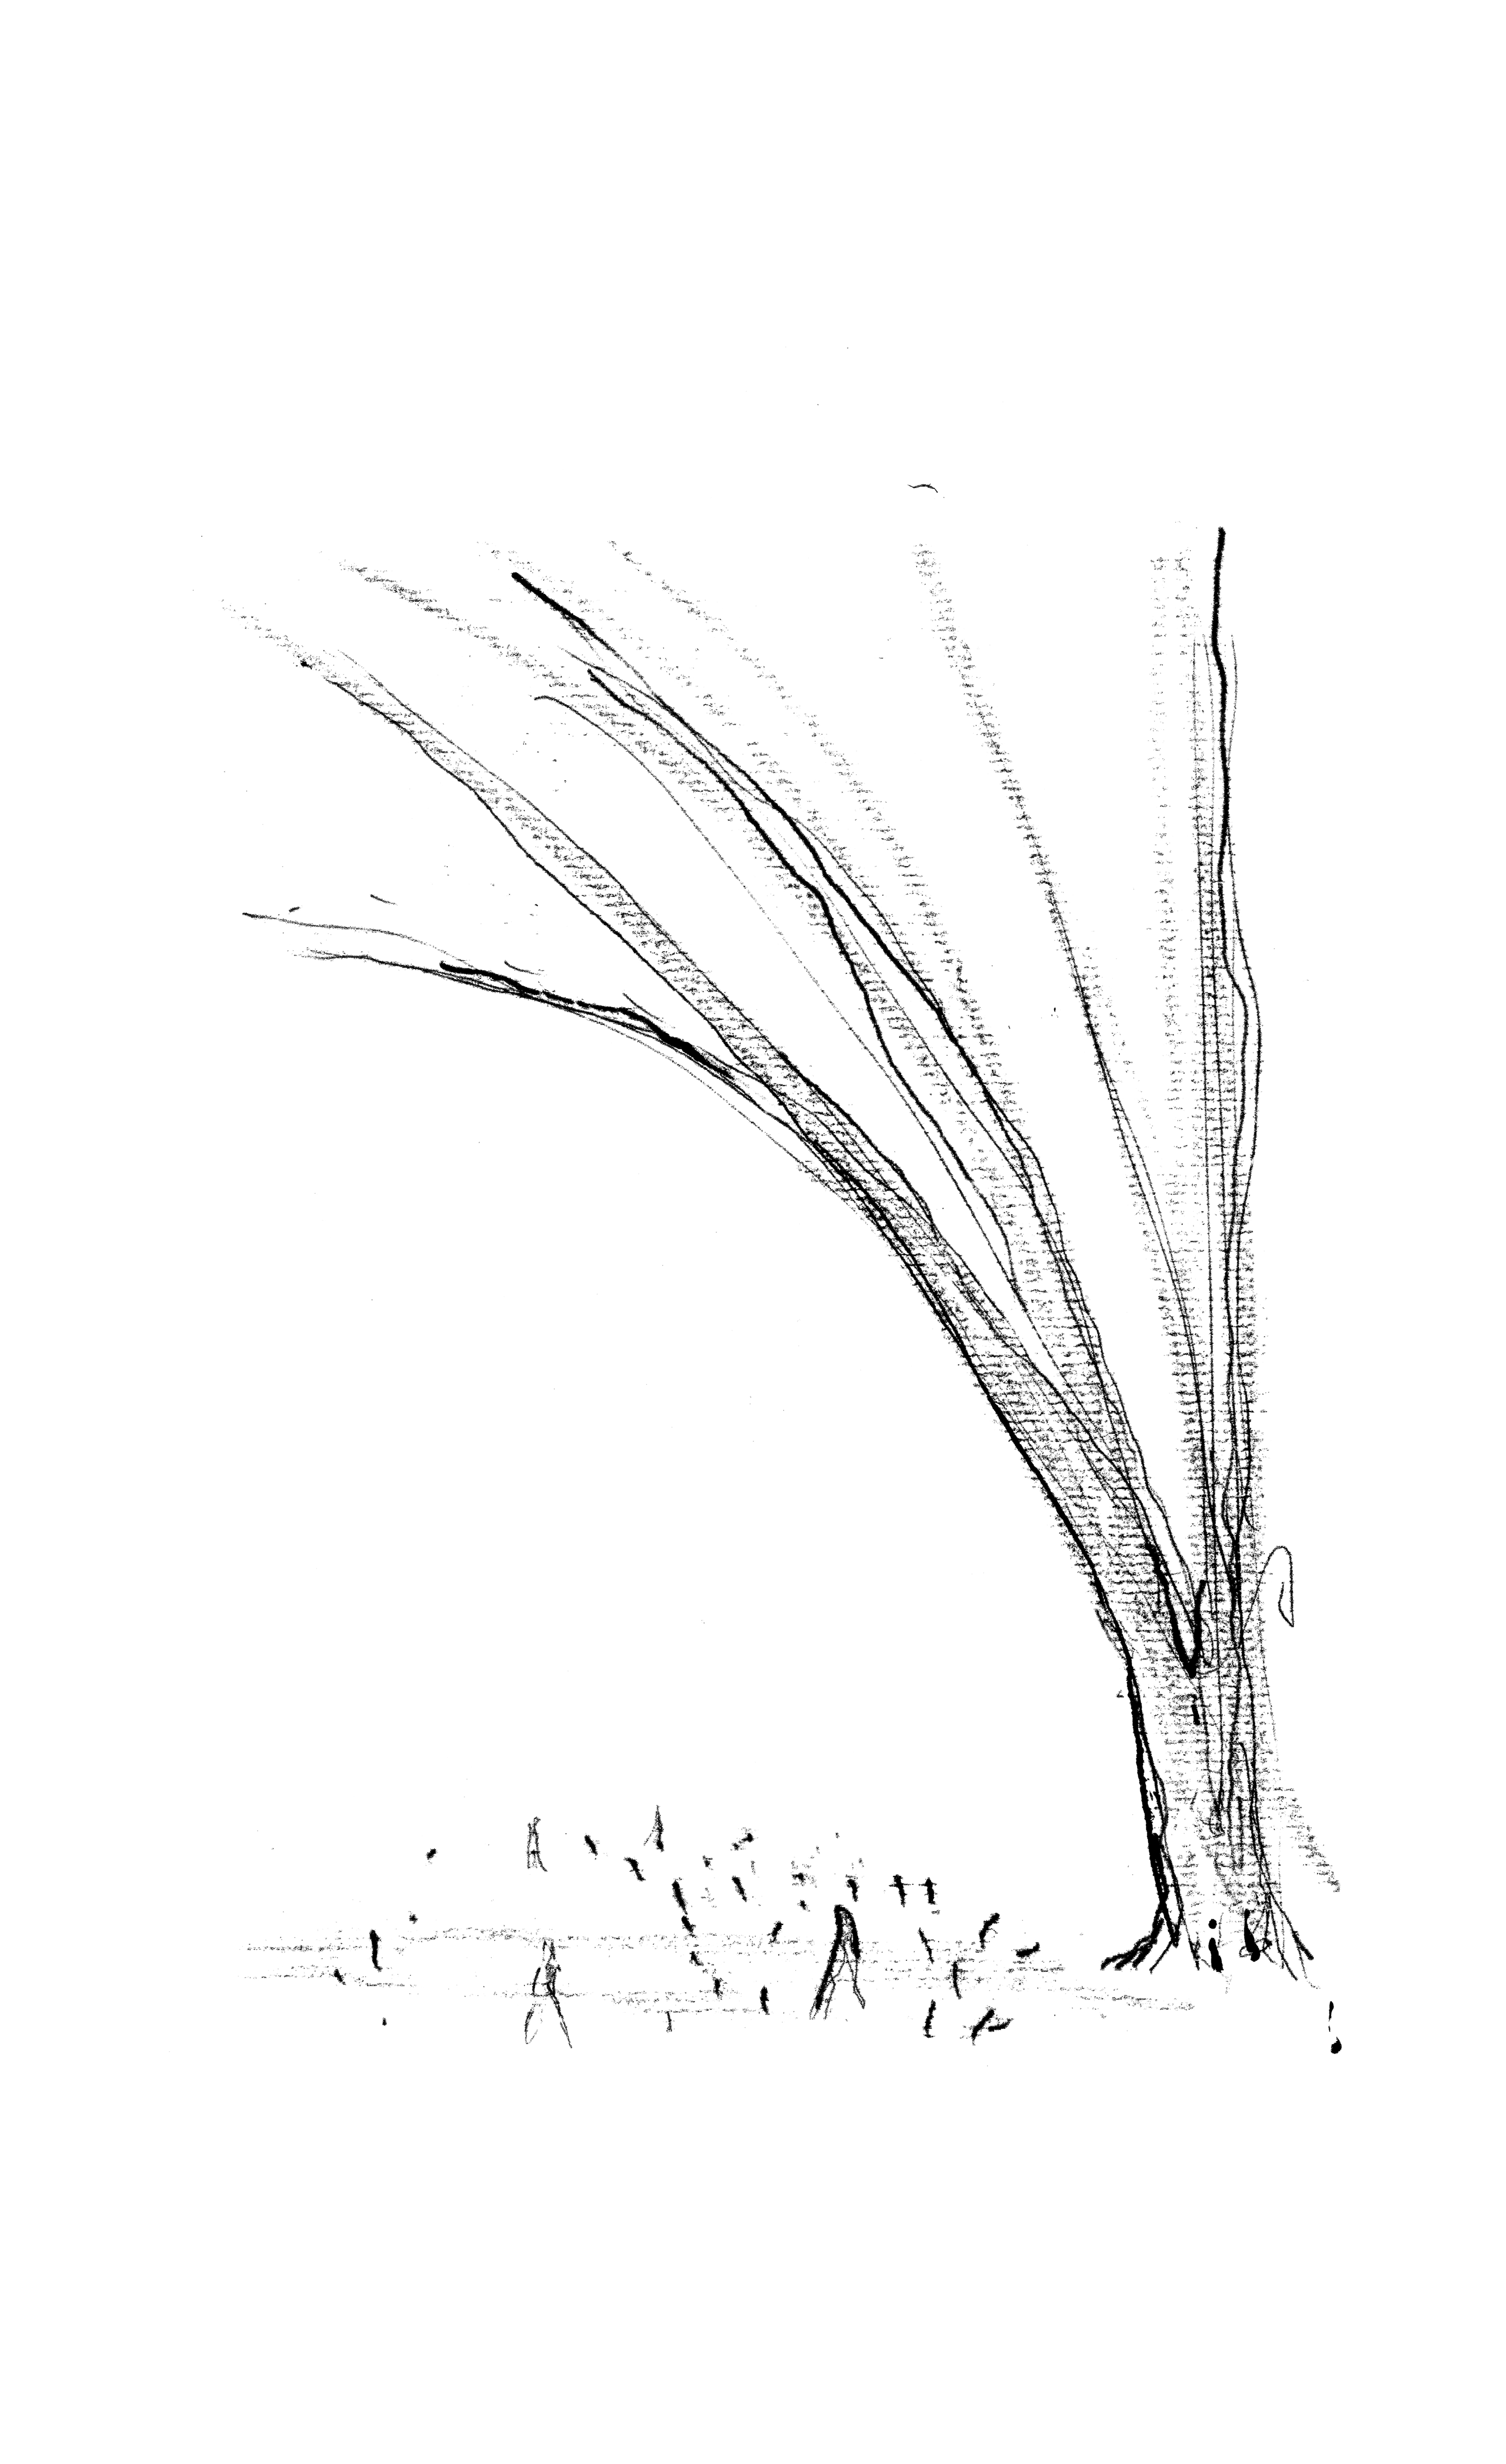
\includegraphics[width=111mm]{./imgs/arvore.jpg}
%\end{center}
%%\end{vplace}

\movetooddpage
\section{xxii}

Não são os desenlaces que me assustam, mas a tentativa de os evitar. Sempre que
senti que algo estava para acabar --- um amor, uma situação, um pacto
íntimo comigo mesmo ou com os outros ---, pegava o meu chapéu e ia embora.
A vida tem reservas suficientes para não tropeçarmos em restos ou
arrependimentos. Sinto"-me incapaz de reparar um gesto ou uma palavra, de
modificar algo que já foi, de retomá"-lo do início e repeti"-lo
com atenção redobrada, para que possa durar hoje aquilo que quebrou
ontem.

``Você é mau?'', pergunta E., baseando"-se em suas pobres nostalgias
contrariadas. Não sou capaz de responder nem mesmo com o pouco que
lhe bastaria, uma palavra nebulosa de protesto.

Não. Não sou mau. (Ou não sou só mau.) Mas não consigo remendar algo,
não importa o quê, um objeto ou um sentimento, a partir do momento em
que sua integridade tenha sido minimamente violada. Uma mancha, uma
sombra, uma opinião basta para um ponto final.

Sempre que tentaram me explicar aquilo a que chamamos ``erro'' (no
texto: \emph{un malentendu}, \textsc{n.~t.}), tiveram razão sobre mim. Jamais tive
a intenção de retrucar e nem tinha como. Os argumentos me desarmam:
todos são bons e todos saem pela culatra. Afinal, que razão pode se opor
a uma pessoa que, como eu, não procura justificativas, mas apenas
significados, sua lei sendo não a de entender, mas a de acreditar?

Tudo pode ser simulado: inteligência, boa fé, virtude, cinismo, até a
verdade. Mas as coisas são puras ou impuras. E isso não se simula nem
se remenda.

\movetooddpage
\section{xxiii}

Se há algo que aprecie no espetáculo da minha própria existência é
uma certa inclinação que julgo especial em reconhecer e aceitar um
milagre. Nada excluo das possibilidades da vida, absolutamente nada, e
aguardo o dia em que o milagre, um milagre, se cumpra. Então ficarei
feliz em não me admirar e em me aproximar dele com descontração, como se
me aproximasse de algo comum e rotineiro.

Às vezes acabo levando a certeza de que algo arrojado deva
acontecer, até às raias do absurdo, ao ponto de condicionar uma
ninharia, uma promessa, um encontro amoroso, à não"-realização do meu
milagre.

Tudo o que faço, tudo o que digo, tudo o que projeto é
prescindível levando"-se em consideração essa espera.

\pagebreak
\thispagestyle{empty}
\movetooddpage
\section{xxiv}

Hoje também passei pelo Louvre, sala 27, diante da mesma tela de
Memling em que identifiquei já há algum tempo um bom exemplo de tudo o
que é contrário à minha sensibilidade.

Não tenho o que dizer dessa \emph{ascensão} de estilo flamengo a não ser
que é demasiado explícita. Tudo está dito, nada está omitido. Eis o
globo terrestre, o santo que levita acima dele, as duas pegadas
inscritas na lama! O milagre se relaciona estreitamente às mãos e aos
pés, para poder ser compreendido num só relance e apalpado para sua
confirmação.

Aqui aprendo mais uma vez aquilo que aprendi já tantas vezes em outras
circunstâncias da vida: uma emoção e um sinal resistem a tudo,
desentendimentos brutais, violações veementes, contradições,
contestações e suspeitas, mas não suportam serem demonstrados.

Posso me submeter ou me revoltar. Mas de modo algum discutir.

Entre o espetáculo do mundo e mim há uma mecha de escuridão e outra de
luz, que preservo intacta, sem aquele sentimento menor a que chamam
curiosidade. Para a vida, isso é suficiente.

\pagebreak
\blankpage
\thispagestyle{empty}